\documentclass[border=12pt]{standalone}
\usepackage[utf8]{inputenc}
\usepackage[T1]{fontenc}
\usepackage{tikz}
\usetikzlibrary{arrows.meta, calc, decorations.pathreplacing, positioning, shapes}

% === Muted color palette (shared across both diagrams) ===
% Base grays
\definecolor{darkslate}{HTML}{2D3748}
\definecolor{slate}{HTML}{4A5568}
\definecolor{lightgray}{HTML}{EDF2F7}

% Accent blues
\definecolor{accentblue}{HTML}{3182CE}
\definecolor{lightblue}{HTML}{EBF4FF}

% Accent greens
\definecolor{accentgreen}{HTML}{38A169}
\definecolor{lightgreen}{HTML}{F0FFF4}

% Accent orange
\definecolor{accentorange}{HTML}{DD6B20}
\definecolor{lightorange}{HTML}{FFFAF0}

% Accent purple
\definecolor{accentpurple}{HTML}{805AD5}
\definecolor{lightpurple}{HTML}{FAF5FF}

\begin{document}

% --- Diagram 1: Scale Progression ---
% Diagram 1: Scale Progression — "From Instrument to Planetary Science"
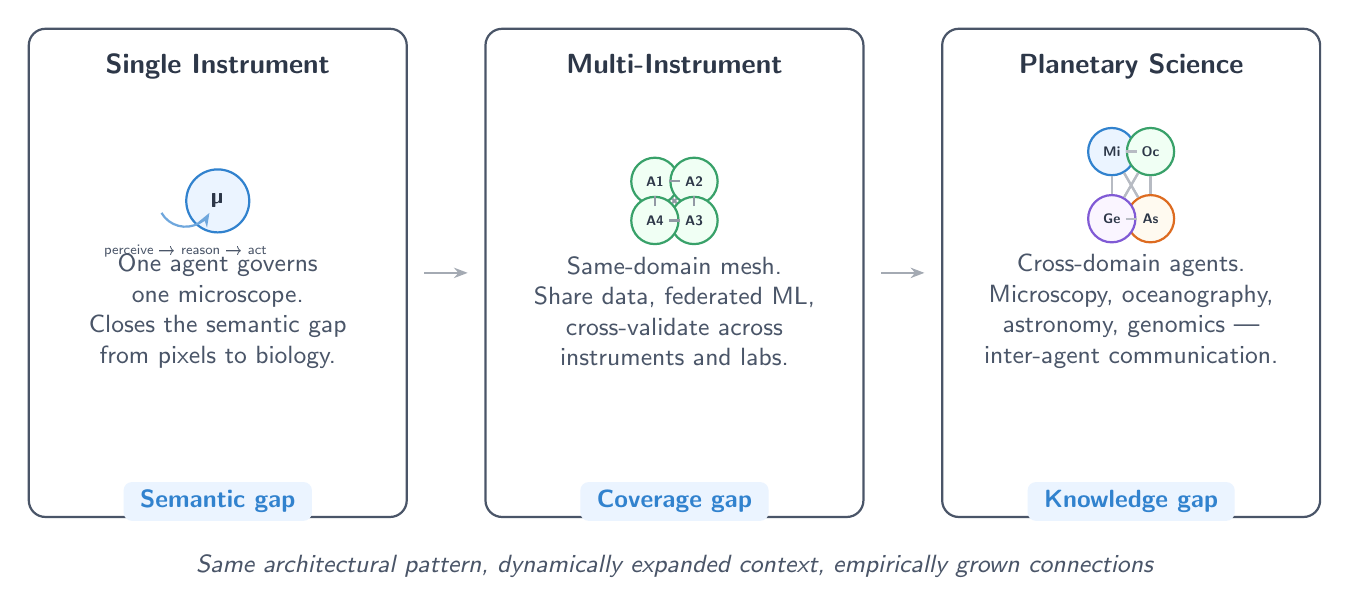
\begin{tikzpicture}[
    remember picture,
    panel/.style={
        draw=slate, thick, rounded corners=6pt,
        minimum width=4.8cm, minimum height=6.2cm,
        fill=white, anchor=north
    },
    paneltitle/.style={
        font=\sffamily\bfseries\normalsize, text=darkslate
    },
    paneldesc/.style={
        font=\sffamily\small, text=slate,
        text width=4cm, align=center
    },
    gaplabel/.style={
        font=\sffamily\small\itshape, text=accentblue,
        fill=lightblue, rounded corners=3pt,
        inner xsep=6pt, inner ysep=3pt
    },
    iconnode/.style={
        draw=accentblue, thick, circle,
        minimum size=8mm, fill=lightblue,
        font=\sffamily\footnotesize\bfseries, text=darkslate
    },
    agentnode/.style={
        draw=accentgreen, thick, circle,
        minimum size=6mm, fill=lightgreen,
        font=\sffamily\tiny\bfseries, text=darkslate
    },
    meshline/.style={
        draw=slate!60, thick
    },
    arrowbridge/.style={
        -{Stealth[length=5pt]}, thick, draw=slate!50
    },
]

% === Color definitions (if not already defined) ===
% Defined in main.tex

% === Panel positions ===
\coordinate (p1) at (0, 0);
\coordinate (p2) at (5.8, 0);
\coordinate (p3) at (11.6, 0);

% === Panel 1: Single Instrument ===
\node[panel] (panel1) at (p1) {};
\node[paneltitle, anchor=north] at ([yshift=-6pt]panel1.north) {Single Instrument};

% Microscope icon — stylized
\node[iconnode] (mic1) at ([yshift=-2.2cm]panel1.north) {\footnotesize\textmu};

% Agent loop arrows
\draw[arrowbridge, draw=accentblue!70]
    ([xshift=-12pt, yshift=4pt]mic1.south west)
    arc[start angle=210, end angle=330, radius=10pt]
    node[midway, below=3pt, font=\sffamily\tiny, text=slate] {perceive \textrightarrow\ reason \textrightarrow\ act};

% Description
\node[paneldesc] at ([yshift=-3.6cm]panel1.north) {
    One agent governs\\one microscope.\\Closes the semantic gap\\from pixels to biology.
};

% Gap label
\node[gaplabel] at ([yshift=6pt]panel1.south) {\textbf{Semantic gap}};

% === Panel 2: Multi-Instrument ===
\node[panel] (panel2) at (p2) {};
\node[paneltitle, anchor=north] at ([yshift=-6pt]panel2.north) {Multi-Instrument};

% Mesh of 4 nodes
\foreach \i/\a in {1/135, 2/45, 3/-45, 4/-135} {
    \node[agentnode] (m\i) at ([shift=(\a:10pt), yshift=-2.2cm]panel2.north) {A\i};
}
% Mesh edges
\foreach \i in {1,2,3,4} {
    \foreach \j in {1,2,3,4} {
        \ifnum\i<\j
            \draw[meshline] (m\i) -- (m\j);
        \fi
    }
}

% Description
\node[paneldesc] at ([yshift=-3.6cm]panel2.north) {
    Same-domain mesh.\\Share data, federated ML,\\cross-validate across\\instruments and labs.
};

% Gap label
\node[gaplabel] at ([yshift=6pt]panel2.south) {\textbf{Coverage gap}};

% === Panel 3: Planetary Science ===
\node[panel] (panel3) at (p3) {};
\node[paneltitle, anchor=north] at ([yshift=-6pt]panel3.north) {Planetary Science};

% Cross-domain agents — colored by domain
\node[draw=accentblue, thick, circle, minimum size=6mm, fill=lightblue,
      font=\sffamily\tiny\bfseries, text=darkslate]
      (d1) at ([shift=(120:14pt), yshift=-2.0cm]panel3.north) {Mi};
\node[draw=accentgreen, thick, circle, minimum size=6mm, fill=lightgreen,
      font=\sffamily\tiny\bfseries, text=darkslate]
      (d2) at ([shift=(60:14pt), yshift=-2.0cm]panel3.north) {Oc};
\node[draw=accentorange, thick, circle, minimum size=6mm, fill=lightorange,
      font=\sffamily\tiny\bfseries, text=darkslate]
      (d3) at ([shift=(-60:14pt), yshift=-2.0cm]panel3.north) {As};
\node[draw=accentpurple, thick, circle, minimum size=6mm, fill=lightpurple,
      font=\sffamily\tiny\bfseries, text=darkslate]
      (d4) at ([shift=(-120:14pt), yshift=-2.0cm]panel3.north) {Ge};

% Cross-domain edges
\foreach \i in {d1,d2,d3,d4} {
    \foreach \j in {d1,d2,d3,d4} {
        \draw[meshline, draw=slate!40] (\i) -- (\j);
    }
}

% Description
\node[paneldesc] at ([yshift=-3.6cm]panel3.north) {
    Cross-domain agents.\\Microscopy, oceanography,\\astronomy, genomics —\\inter-agent communication.
};

% Gap label
\node[gaplabel] at ([yshift=6pt]panel3.south) {\textbf{Knowledge gap}};

% === Bridging arrows between panels ===
\draw[arrowbridge, shorten >=4pt, shorten <=4pt]
    ([xshift=2pt]panel1.east) -- ([xshift=-2pt]panel2.west);
\draw[arrowbridge, shorten >=4pt, shorten <=4pt]
    ([xshift=2pt]panel2.east) -- ([xshift=-2pt]panel3.west);

% === Tagline ===
\node[font=\sffamily\small\itshape, text=slate, anchor=north]
    at ([yshift=-10pt]panel2.south) {
    Same architectural pattern, dynamically expanded context, empirically grown connections
};

\end{tikzpicture}


\newpage

% --- Diagram 2: Domain Map ---
% Diagram 2: Gently Domain Map — "Domains of the Agentic Microscope"
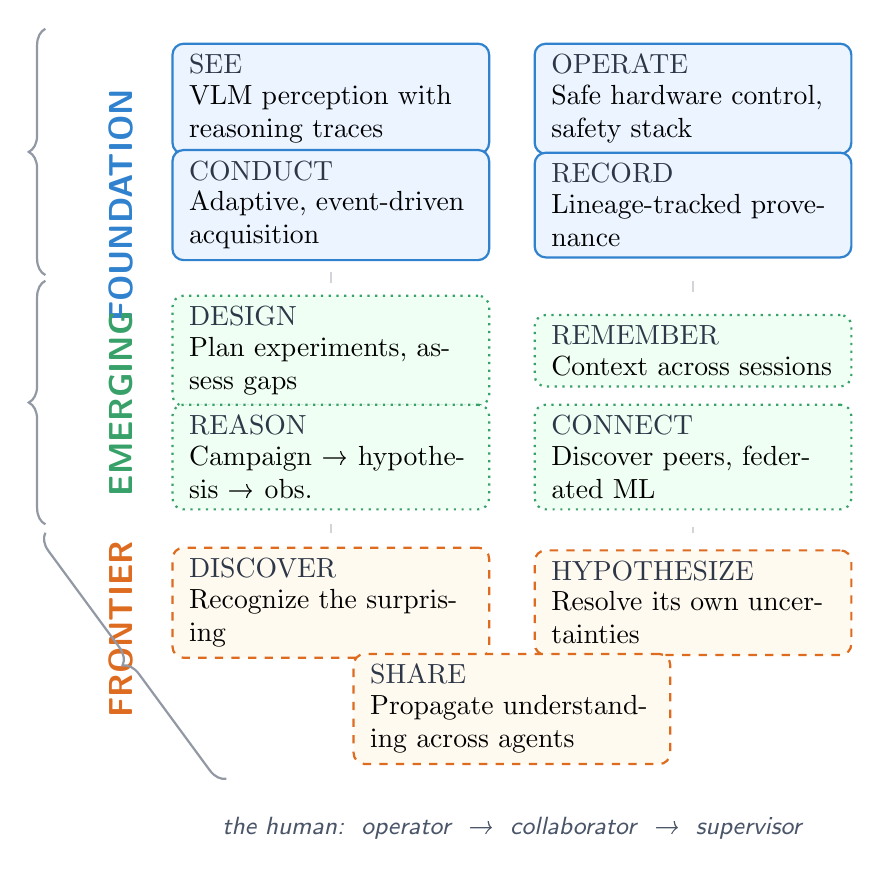
\begin{tikzpicture}[
    remember picture,
    % Tier styles
    foundationbox/.style={
        draw=accentblue, thick, rounded corners=4pt,
        fill=lightblue, minimum height=9mm,
        text width=3.6cm, align=left,
        inner xsep=6pt, inner ysep=4pt
    },
    emergingbox/.style={
        draw=accentgreen, thick, dotted, rounded corners=4pt,
        fill=lightgreen, minimum height=9mm,
        text width=3.6cm, align=left,
        inner xsep=6pt, inner ysep=4pt
    },
    frontierbox/.style={
        draw=accentorange, thick, dashed, rounded corners=4pt,
        fill=lightorange, minimum height=9mm,
        text width=3.6cm, align=left,
        inner xsep=6pt, inner ysep=4pt
    },
    verblabel/.style={
        font=\sffamily\bfseries\normalsize
    },
    desclabel/.style={
        font=\sffamily\small, text=slate
    },
    tierlabel/.style={
        font=\sffamily\bfseries\large, rotate=90, anchor=south
    },
    tierbrace/.style={
        decorate, decoration={brace, amplitude=6pt, mirror}, thick, draw=slate!60
    },
]

% Layout parameters
\def\colsep{4.6cm}
\def\rowsep{1.35cm}
\def\tierpad{0.3cm}

% === FOUNDATION tier ===
\node[tierlabel, text=accentblue] at (-2.4, -0.5*\rowsep - 0.5*\rowsep) {FOUNDATION};

\node[foundationbox] (see) at (0, 0) {
    \textcolor{darkslate}{\verblabel SEE}\\[-1pt]
    {\desclabel VLM perception with reasoning traces}
};
\node[foundationbox] (operate) at (\colsep, 0) {
    \textcolor{darkslate}{\verblabel OPERATE}\\[-1pt]
    {\desclabel Safe hardware control, safety stack}
};
\node[foundationbox] (conduct) at (0, -\rowsep) {
    \textcolor{darkslate}{\verblabel CONDUCT}\\[-1pt]
    {\desclabel Adaptive, event-driven acquisition}
};
\node[foundationbox] (record) at (\colsep, -\rowsep) {
    \textcolor{darkslate}{\verblabel RECORD}\\[-1pt]
    {\desclabel Lineage-tracked provenance}
};

% Foundation brace
\draw[tierbrace]
    ([xshift=-1.6cm, yshift=5pt]see.north west) --
    ([xshift=-1.6cm, yshift=-5pt]conduct.south west);

% === EMERGING tier ===
\def\emergingstart{-3.2cm}
\node[tierlabel, text=accentgreen] at (-2.4, \emergingstart - 0.5*\rowsep) {EMERGING};

\node[emergingbox] (design) at (0, \emergingstart) {
    \textcolor{darkslate}{\verblabel DESIGN}\\[-1pt]
    {\desclabel Plan experiments, assess gaps}
};
\node[emergingbox] (remember) at (\colsep, \emergingstart) {
    \textcolor{darkslate}{\verblabel REMEMBER}\\[-1pt]
    {\desclabel Context across sessions}
};
\node[emergingbox] (reason) at (0, \emergingstart - \rowsep) {
    \textcolor{darkslate}{\verblabel REASON}\\[-1pt]
    {\desclabel Campaign \textrightarrow\ hypothesis \textrightarrow\ obs.}
};
\node[emergingbox] (connect) at (\colsep, \emergingstart - \rowsep) {
    \textcolor{darkslate}{\verblabel CONNECT}\\[-1pt]
    {\desclabel Discover peers, federated ML}
};

% Emerging brace
\draw[tierbrace]
    ([xshift=-1.6cm, yshift=5pt]design.north west) --
    ([xshift=-1.6cm, yshift=-5pt]reason.south west);

% === FRONTIER tier ===
\def\frontierstart{-6.4cm}
\node[tierlabel, text=accentorange] at (-2.4, \frontierstart - 0.25*\rowsep) {FRONTIER};

\node[frontierbox] (discover) at (0, \frontierstart) {
    \textcolor{darkslate}{\verblabel DISCOVER}\\[-1pt]
    {\desclabel Recognize the surprising}
};
\node[frontierbox] (hypothesize) at (\colsep, \frontierstart) {
    \textcolor{darkslate}{\verblabel HYPOTHESIZE}\\[-1pt]
    {\desclabel Resolve its own uncertainties}
};
\node[frontierbox] (share) at (0.5*\colsep, \frontierstart - \rowsep) {
    \textcolor{darkslate}{\verblabel SHARE}\\[-1pt]
    {\desclabel Propagate understanding across agents}
};

% Frontier brace
\draw[tierbrace]
    ([xshift=-1.6cm, yshift=5pt]discover.north west) --
    ([xshift=-1.6cm, yshift=-5pt]share.south west);

% === Thin connecting lines between tiers ===
\draw[draw=slate!25, thick]
    ([yshift=-8pt]conduct.south) -- ([yshift=8pt]design.north);
\draw[draw=slate!25, thick]
    ([yshift=-8pt]record.south) -- ([yshift=8pt]remember.north);
\draw[draw=slate!25, thick]
    ([yshift=-8pt]reason.south) -- ([yshift=8pt]discover.north);
\draw[draw=slate!25, thick]
    ([yshift=-8pt]connect.south) -- ([yshift=8pt]hypothesize.north);

% === Footer ===
\node[font=\sffamily\small\itshape, text=slate, anchor=north]
    at (0.5*\colsep, \frontierstart - 2*\rowsep + 0.1cm) {
    the human:\ \ operator\ \ \textrightarrow\ \ collaborator\ \ \textrightarrow\ \ supervisor
};

\end{tikzpicture}


\end{document}
